%!TEX root = ./main.tex
%
% This file is part of the i10 thesis template developed and used by the
% Media Computing Group at RWTH Aachen University.
% The current version of this template can be obtained at
% <http://www.media.informatik.rwth-aachen.de/karrer.html>.

\chapter{Evaluation}
\label{evaluation}
\index{evaluation|(}

In this chapter we will evaluate our prototypes with respect to the quantitative and qualitative aspects of the different feedback methods. We are interested to what extent the perception of feedback differs onshore versus underwater regarding time until the stimulus is perceived. 
We conducted a user study consisting of two parts: in the first part we measured reaction times between presentation of the feedback and it being perceived by the user.
The second part was a questionnaire investigating preferences and experiences regarding the feedback types and their applicability for navigation under water. 
  

\section{User Study}

The apparatus consists of a button at the edge of the pool, diving goggles with an LED on the right side, a headband with a vibration motor and a thermoelectric cooler (TEC), and waterproof in-ear headphones. 
These are encapsulated and connected to an Arduino Uno except for the headphones which are directly connected to the MacBook Pro. 
The Arduino measures the time between the activation of a feedback and the press of the button. 
For sound the Arduino sends the command to Processing which then plays the sound file and measures the reaction time. 
Processing logs the time in milliseconds and the corresponding feedback for further analysis.

\subsection{Procedure}
The participants took a shower and were asked to swim a few laps until they felt at ease. 
They put on the diving goggles and the headband first, and we ensured that the TEC had direct contact to the skin and that the headband was worn firmly and comfortably. 
Finally, participants put on the snorkel and the earphones. Then the participant was instructed to submerge, start the study by pressing the button for the first time, and press the button as soon as she perceives a stimulus (Fig. 2). 
Every run included each stimulus eight times in random order with the same stimulus being repeated at most two times in a row. After the button was pressed the next stimulus was randomly delayed between two and eight seconds to prevent adaption. 
This was repeated at least four times per participant with some participants voluntarily doing more runs. 
Participants were allowed to emerge anytime they feel uncomfortable or had issues with the equipment. 
Afterwards, participants answered questions on a 5-point Likert scale regarding feedback recognition, feedback comfort, and imagining the feedback type for underwater navigation.

\subsection{Design}
The independent variable was STIMULUS (simple LED, pulsing LED, vibration, increasing vibration, cooling, sound). 
A sequence of eight stimuli of each type in random order for each run and at least 4 runs per user resulted in (6 x 8 x 4) 192 trials per user in a within-subjects design (48 trials for every additional run). 
The dependent variable is Time [ms] which denoted the time between a stimulus started and the button was pressed.

\subsection{Results}
\begin{figure}
	\centering
	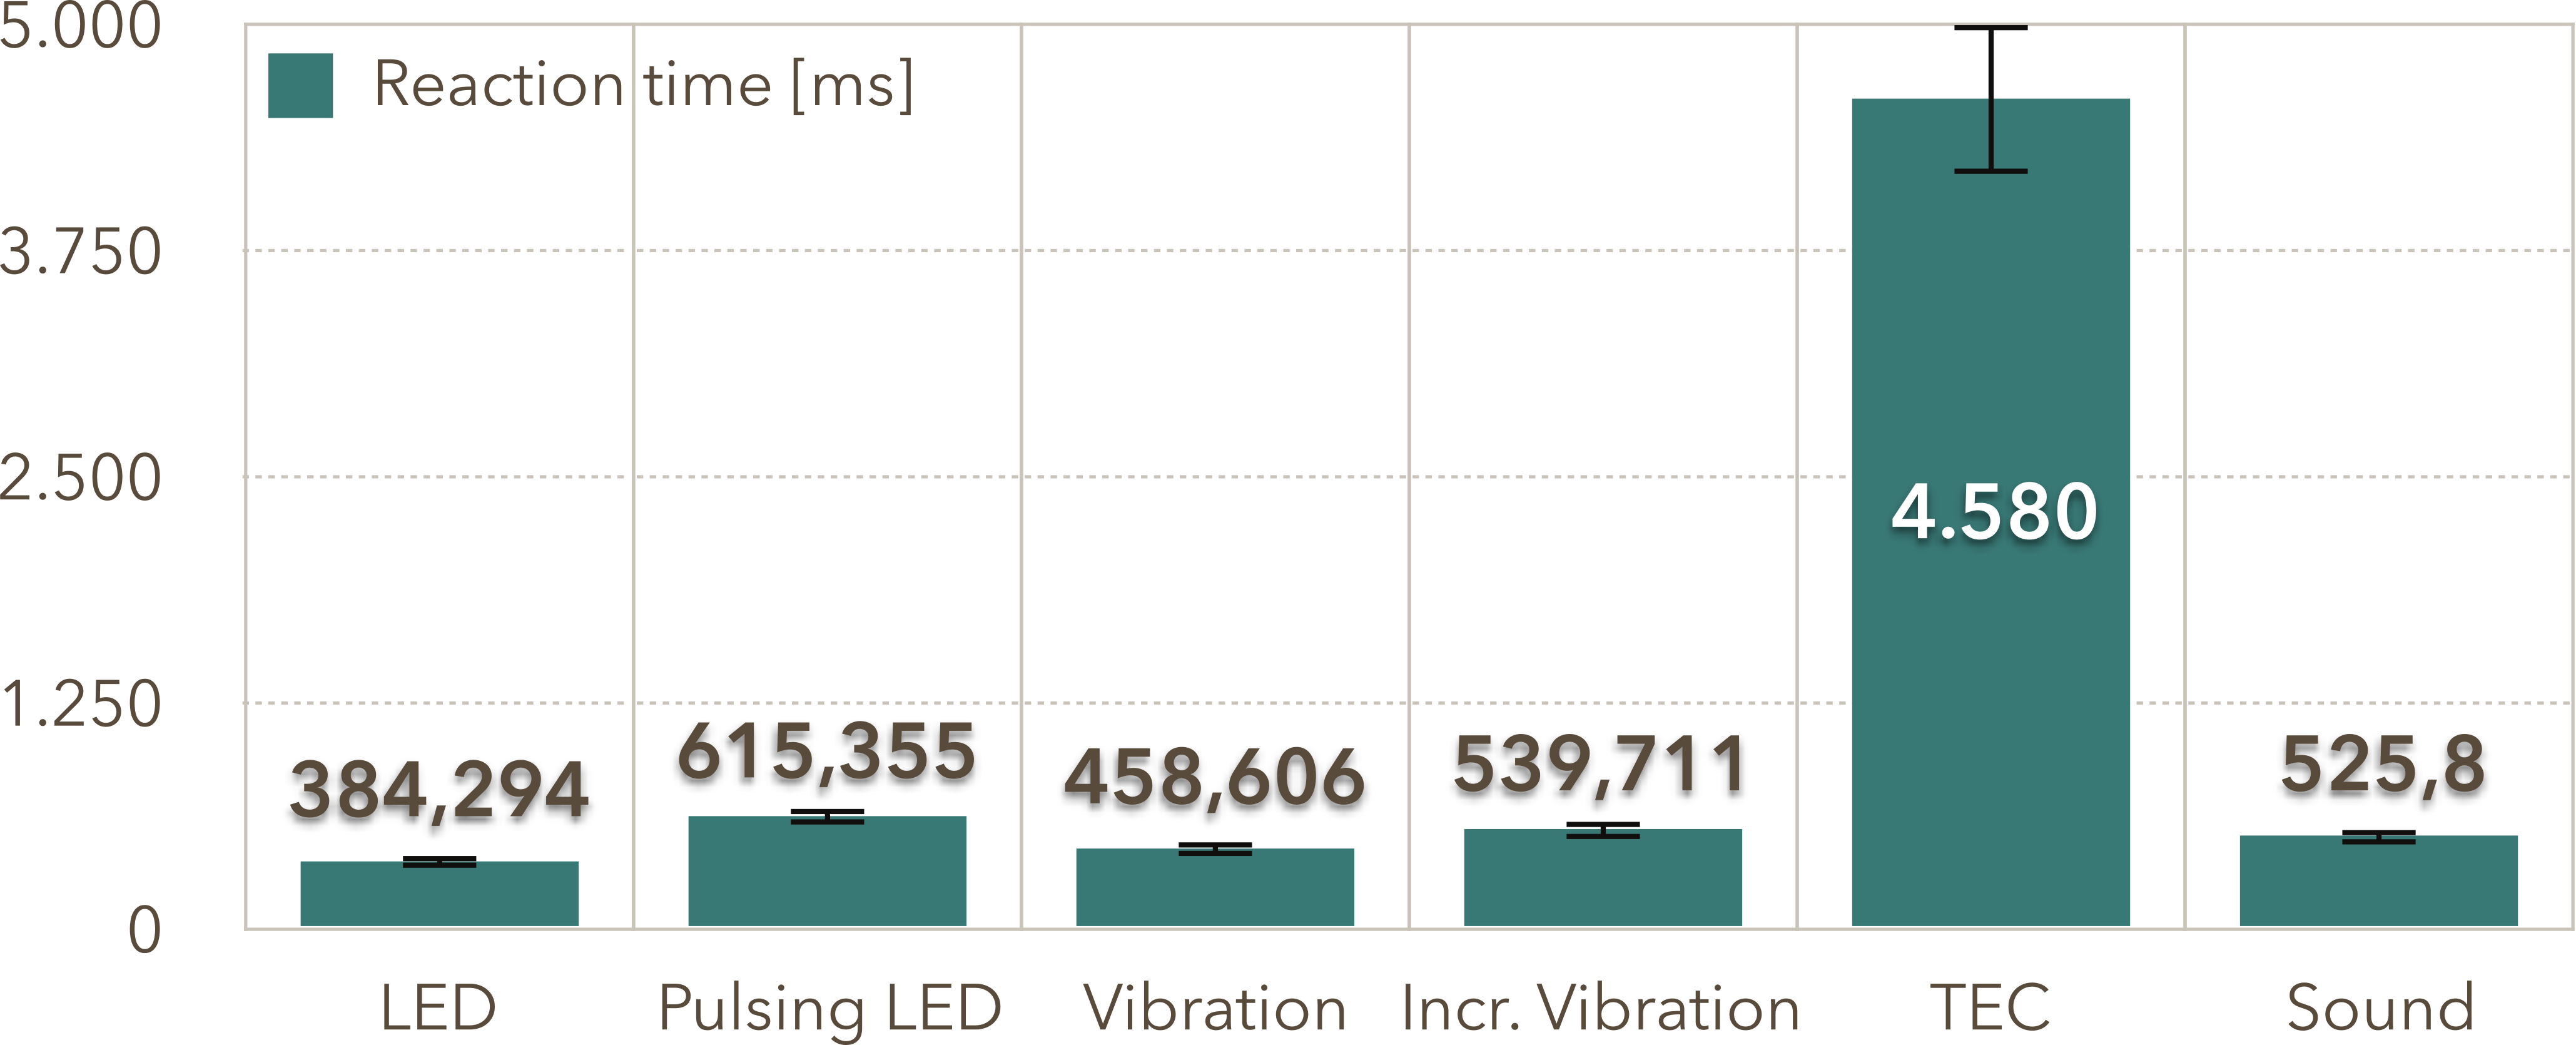
\includegraphics[width=\columnwidth]{images/ResultsOfReactionTimes}
	\caption{Results of the reaction time on different feedback types under water. Means and 95\% confidence intervals.}~\label{fig:reactiontimes}
	\vspace{-2em}
\end{figure}

\begin{figure}
	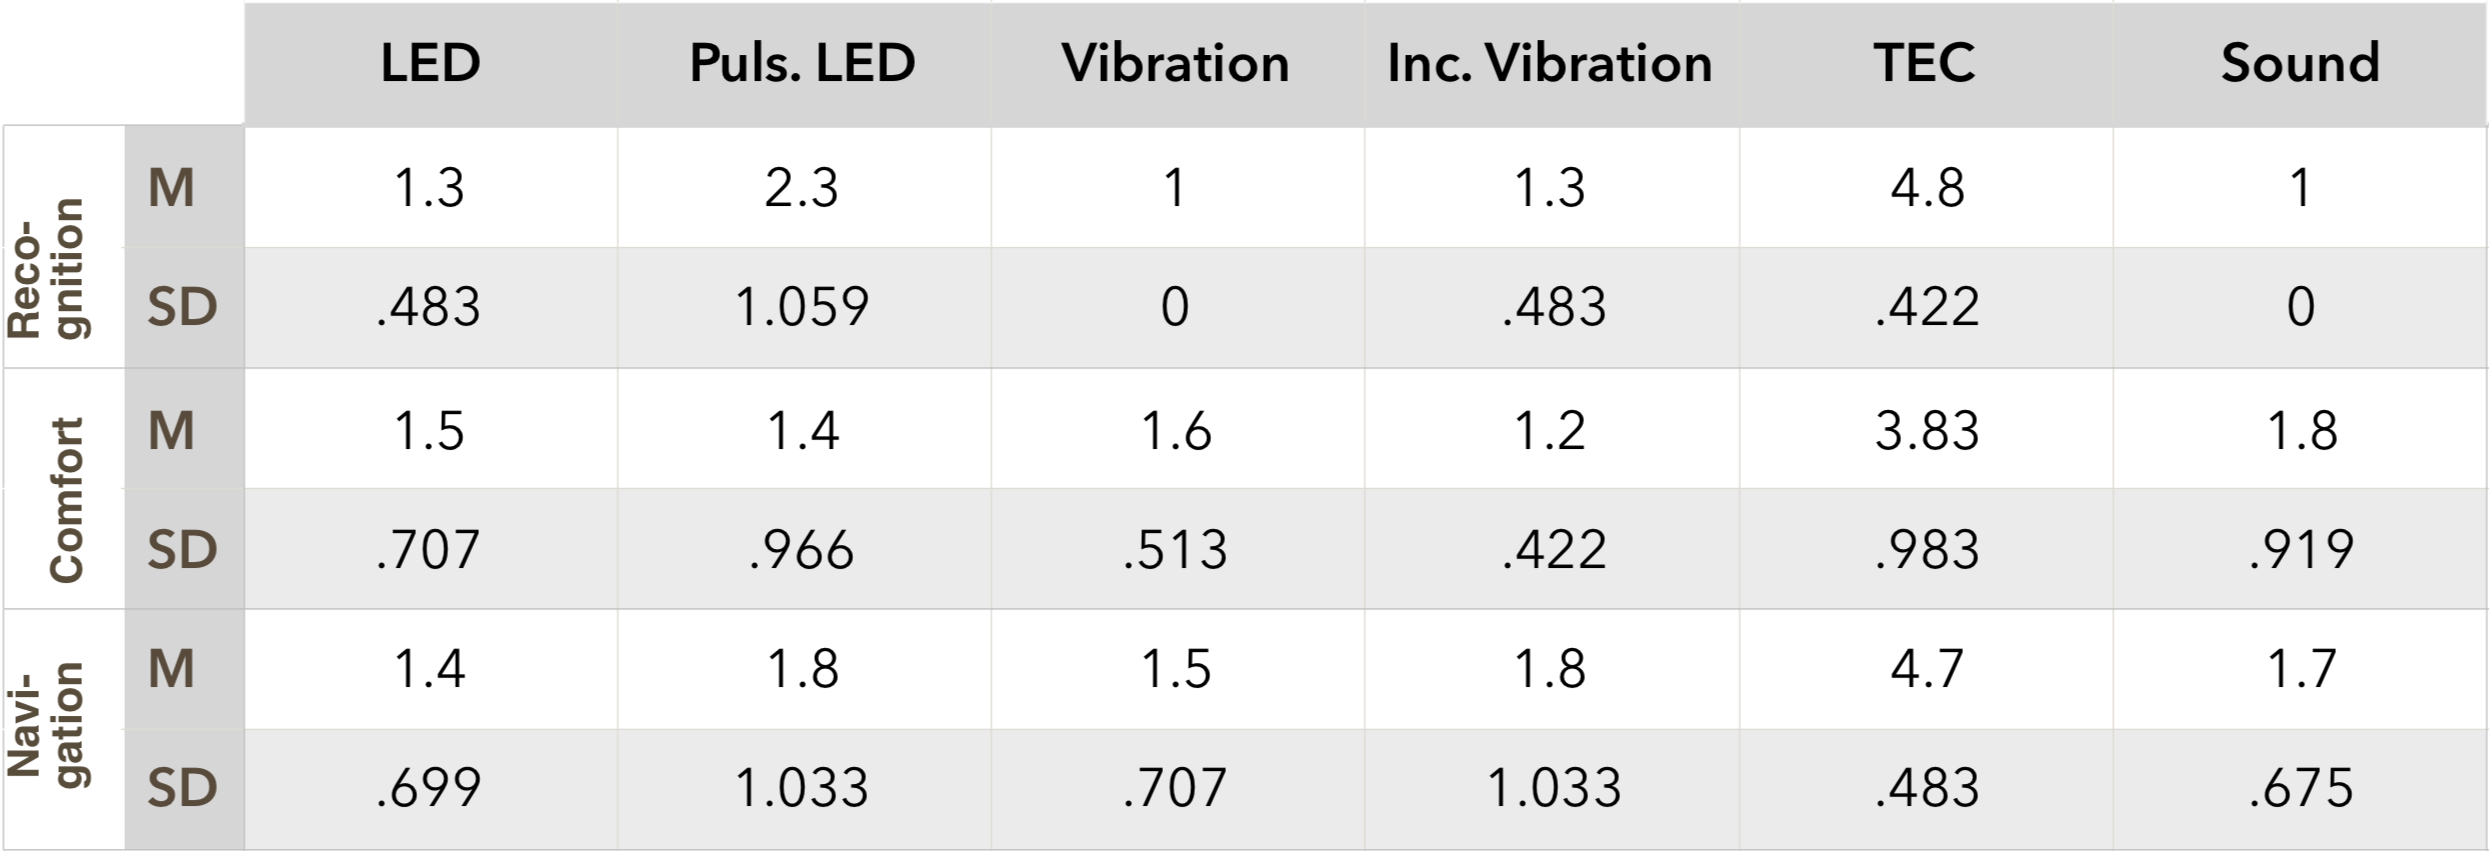
\includegraphics[width=\columnwidth]{images/m_sd_table_noranking}
	\caption{Means and standard deviations (less is better) of the results from the questionnaire.}~\label{fig:m_sd_table}
\end{figure}

A total of 10 users participated in the study (average age 24.1, 8 male), five of which had prior experience with diving or snorkeling. 
391 outliers (results differed by more than 1.5 SD from the mean) were identified resulting in 2021 data points. 
Only 4 participants recognized the TEC at all which led to the majority of outliers. 
The remaining outliers are caused by issues with the equipment (e.g., water in the snorkel or goggles), forcing the participant to emerge.
We log-transformed \emph{Time} for a repeated measures ANOVA. 
{\sc stimulus} had a significant effect on \emph{Time} ($F\textsubscript{1991} = 852.97, p<.0001$). 
Tukey HSD post hoc pairwise comparisons showed that the TEC (4580$ms$) was significantly slower compared to each other {\sc stimulus} and pulsing LED (615$ms$) was significantly slower than vibration (458$ms$) and simple LED (384$ms$).

We used Friedman and Wilcoxon Signed Ranks tests to evaluate the questionnaire (cf.\ Table~\ref{fig:m_sd_table}).
There was a significant difference in user rated recognition ($\chi^2$(5) = 39.73, $p<.001$).
Post-hoc pairwise comparison revealed that the TEC was perceived significantly less than all other stimuli ($p<.005$). \newline
There was a significant difference in user rated comfort ($\chi^2$(5) = 15.83, $p<.007$).
Post-hoc pairwise comparison revealed that TEC was significantly less comfortable than all other stimuli ($p<.041$) and increasing vibration was significantly more comfortable than vibration ($p<.046$). \newline
There was a significant difference in user rated navigation suitability ($\chi^2$(5) = 28.77, $p<.001$). 
Post-hoc pairwise comparison revealed that only the TEC was rated significantly less suitable for underwater navigation ($p<.004$).

\subsection{Discussion}
The results and the tremendous power consumption show that the TEC is not suitable for underwater applications. 
Partici- pants reported that it is hard to tell whether the TEC is active or if it is a cold flow of water. 
The skin adapts to thermal changes quickly and makes consecutive cooling events hard to detect [6]. 
Visual, vibrotactile, and auditory stimuli are suit- able for underwater navigation regarding reaction time (384 - 615ms). 
Even though the LED feedback was fastest (384ms) the vibration (459ms) was perceived to be recognized faster. 
Binary feedback using light and vibration is perceived as less comfortable than the fading counterparts. 
Therefore, in an un- derwater navigation scenario, instant feedback should be used for time critical events only. 
Otherwise, the more comfortable stimuli suffice. 
Participants commented that LED feedback can be mistaken for water reflections or to be obstructive and distracting. 
Sound was rated as being immediately perceiv- able (1.0), but some users felt uncomfortable wearing in-ear headphones under water. 
Vibration on the other hand uses a different sense which is not occupied while diving/snorkeling and provides clear and comfortable feedback. 
Furthermore, vibration feedback acts like bone conductance sound, and therefore, also includes additional auditory feedback.

\subsection{Testing outside the water}

We let one user test it outside the water to get a rough estimate how the medium influences the results in general.
This user is sitting on a table and wears the prototype including the diving goggles but without the snorkel.
The relay we use makes a notable clicking noise which is audible through the headphones worn by the participant.
Therefore we use a pillow and a wastebin to make it infrasonic.
Again we let the user do as many trials as she was willing to do.
210 trials are carried out by the user.
Other than that the procedure and the user study program remain the same as described above.

The results of the participant is shown in figure~\ref{fig:user12}.
It is immediately notable that the visual stimulus is on average faster received in the under water condition (LED: 69.285 ms, Pulsing LED: 81.708 ms).
Contrarily to the visual modality on average the haptic feedback of the vibration motor is faster perceived outside the water (Vibration: 28.822 ms, Increasing Vibration: 109.135 ms).
The most preeminent difference between the two mediums is measured when it comes to thermal feedback.
Not only is the cooling effect of the peltier element recognized reliably by the participant, but also 3152.580 ms faster with 1427.657 ms.
Sound was perceived negligibly faster underwater with 19.339 ms difference.

\begin{figure}
	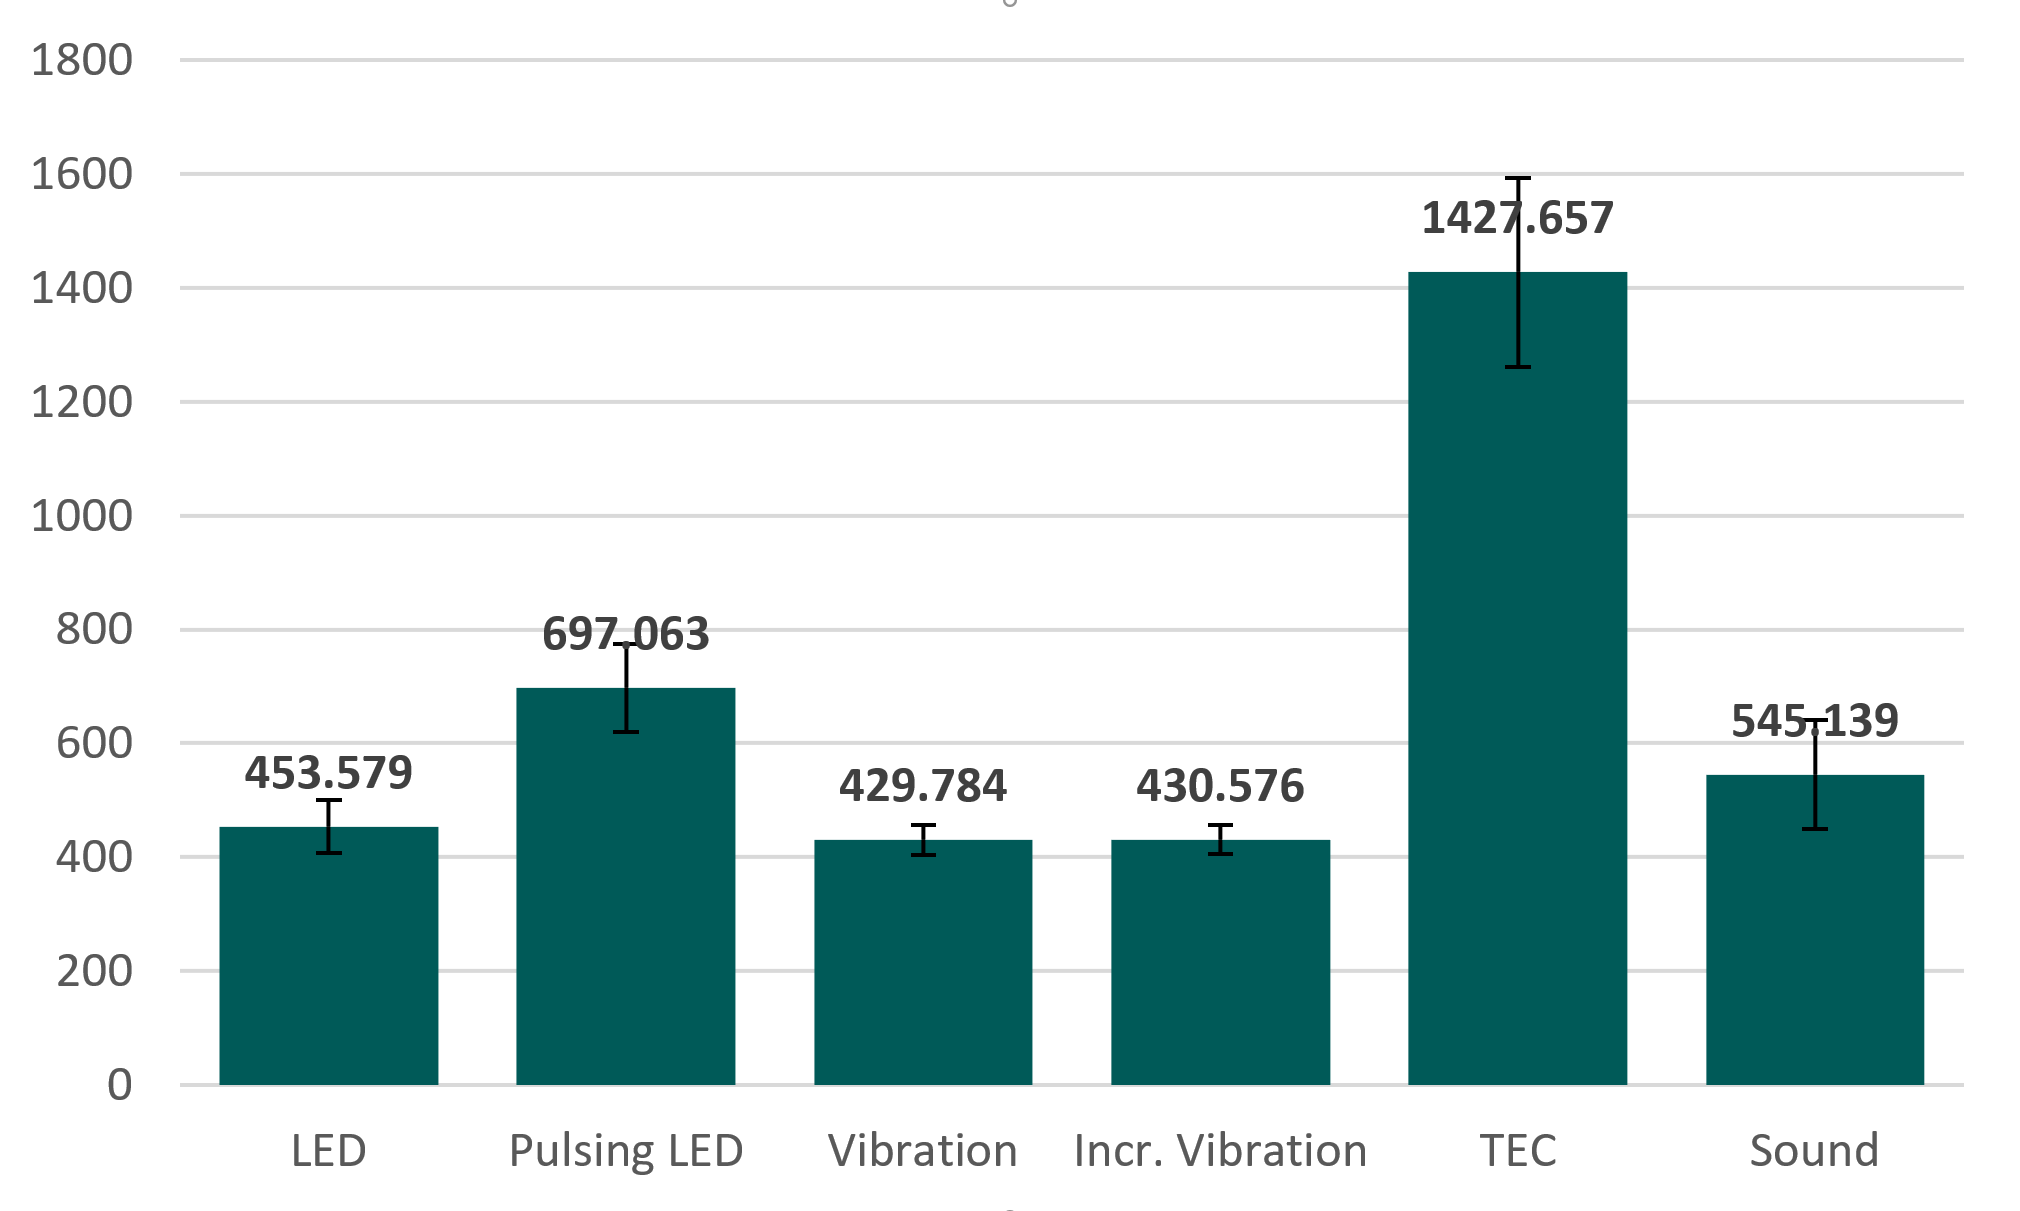
\includegraphics[width=\columnwidth]{images/ResultsOfReactionTimesUser12.png}
	\caption{Results of the reaction time on different feedback types ashore. Means and 95\% confidence intervals. }~\label{fig:user12}
\end{figure}
\index{evaluation|)}






























